\documentclass{beamer}
%
% Choose how your presentation looks.
%
% For more themes, color themes and font themes, see:
% http://deic.uab.es/~iblanes/beamer_gallery/index_by_theme.html
%
\mode<presentation>
{
  \usetheme{default}      % or try Darmstadt, Madrid, Warsaw, ...
  \usecolortheme{default} % or try albatross, beaver, crane, ...
  \usefonttheme{default}  % or try serif, structurebold, ...
  \setbeamertemplate{navigation symbols}{}
  \setbeamertemplate{caption}[numbered]
} 

\usepackage[english]{babel}
\usepackage[utf8x]{inputenc}
\usepackage{physics}
\usepackage{amsmath}
\usepackage{graphicx}
\usepackage{adjustbox}
\usepackage{wrapfig}
\usepackage[T1]{fontenc}
\usepackage{mdframed}
\usepackage{algorithm}
\usepackage[noend]{algpseudocode}

\definecolor{codegreen}{rgb}{0,0.6,0}
\definecolor{codegray}{rgb}{0.5,0.5,0.5}
\definecolor{codepurple}{rgb}{0.58,0,0.82}
\definecolor{backcolour}{rgb}{0.95,0.95,0.92}
\input{insbox}

\newcommand\hideit[1]{%
  \only<0| handout:1>{\mbox{}}%
  \invisible<0| handout:1>{#1}}

\newmdtheoremenv{defi}{Definition}

\usepackage[sorting=none, style=apa]{biblatex}
\bibliography{bibtex} 

\addtobeamertemplate{navigation symbols}{}{%
    \usebeamerfont{footline}%
    \usebeamercolor[fg]{footline}%
    \hspace{1em}%
    \insertframenumber/\inserttotalframenumber
}

\title[]{Fast Approximations of Quantifier Elimination}
\subtitle{Isabel Garcia-Contreras, V. K. Hari Govind, Sharon Shoham, and Arie Gurfinkel}
\author{Johannes Felzmann, TU Wien}
\date{\today}

\AtBeginSection[]
{
    \begin{frame}
        \frametitle{}
        \tableofcontents[currentsection]
    \end{frame}
}

\begin{document}

\begin{frame}
  \titlepage
   \centering
  \text{ \scriptsize Seminar in Formal Methods WS2023}
\end{frame}

% Uncomment these lines for an automatically generated outline.
%\begin{frame}{Outline}
%  \tableofcontents
%\end{frame}

\begin{frame}{Overview}
\tableofcontents
\end{frame}
\section{Motivation}

\begin{frame}{What is Quantifier elimination?}
    \begin{itemize}
        \item concept of simplification
        \item removal of all quantifiers
        \pause
        \item used in many automated reasoning tasks
        \pause
        \item question/answer problem (\cite{QE})
        \begin{itemize}
            \item \textit{There exists an $x$ s.t. \dots}
            \item \textit{There exists such an $x$ when \dots}
        \end{itemize}
    \end{itemize}
\end{frame}



\begin{frame}{Quantifier elimination (qelim)}

\begin{itemize}
  \item program synthesis
  \item exist-forall solving
  \item quantified SMT
  \item Model checking
  \item solving Constrained Horn Clauses
\end{itemize}

\end{frame}


\begin{frame}{Quantifier elimination (qelim)}

Given a quantifier-free (QF) formula $\varphi$ with free variables $v$, quantifier elimination of $\varphi^{\exists}$ is the problem of finding a QF formula $\psi$ with no free variables such that $\psi \equiv \varphi^{\exists}$.
\pause
\vspace{0.5cm}
Examples:

\vspace{0.1cm}

qelim of $\exists x \hspace{2mm} (a \approx x \land f(x) > 3)$ is $f(a) > 3$ 
\pause
\vspace{0.1cm}

qelim of $\exists x \hspace{2mm} (f(x) > 3)$ does not exist 
(it is impossible to restrict f to have at least one value in its range that is greater than 3 without a quantifier)

\end{frame}



\section{The Problem}


\begin{frame}{Quantifier elimination (qelim) - \textbf{The Bad}}

\begin{block}{is double exponentially.....}
\begin{itemize}
  \item effective implementations of quantifier elimination scale still in a doubly exponential fashion
  \item e.g. Cylindrical Algebraic Decomposition (CAD) (\cite{10.1145/1093390.1093393}) doubly exponential in the number of variables
  \pause
  \item other approaches doubly exponential in the number of quantifier alternations
  \pause
  \item $\Longrightarrow$ 2-EXPTIME complexity
\end{itemize}
\end{block}
\end{frame}

\begin{frame}{Quantifier elimination (qelim) - \textbf{The Good}}

\begin{block}{we can approximate it}
\begin{itemize}
  \item called quantifier reductions
  \item relaxation of qelim
  \item might leave some free variables
  \pause
  \item could be possible even when qelim is not
  \item there exist some algorithms with shortcomings
  \pause
  \item $\Longrightarrow$ new algorithm without tolerating some shortcomings
\end{itemize}
\end{block}
\end{frame}


\begin{frame}{Goal}
\begin{itemize}
  \item develop new quantifier reduction algorithm QEL that is relatively fast
  \pause
    \item traditional algorithms are implemented by a series of syntactic rules, operating directly on the syntax of an input formula
    \pause
  \item $\longrightarrow$ key idea: use egraphs
    \pause
  \item implement QEL and MBP using e-graphs inside the SMT solver Z3
\end{itemize}
\end{frame}


\begin{frame}{QELITE in Z3}
      \begin{itemize}
        \item QEL is based on the subst. rule $(\exists x \textbf{ } x \approx t \land \varphi) \equiv \varphi [x \longmapsto t]$
      \pause
      \item QELITE in Z3 naiv implementation $\longrightarrow$ limited
      \begin{itemize}
      \item $\varphi_2 (x,y) \triangleq y \approx f(x) \land x \approx g(y) \land f(x) \approx 6$
      \begin{itemize}
          \item assume $y$ eliminated with $y \approx f(x)$ resulting $x \approx g(f(x)) \land f(x) \approx 6$
          \item problem! $x$ cannot be eliminated $\longrightarrow$ circular
          \item otw. if it is noted that $y \approx 6$ and therefore $(\exists y \text{ } \varphi_2) \triangleq x \approx g(6) \land f(x) \approx 6$ and following $x \approx g(6)$ is used resulting in $f(g(6)) \approx 6$ qelim of $\varphi_2^{\exists}$
      \end{itemize}
        \end{itemize}
        \pause
        \item $\longrightarrow$ use egraphs !!!
        \item egraphs allow eliminating multiple variables together, ensuring that a variable is eliminated if it is equivalent
      \end{itemize}
\end{frame}

\begin{frame}{Egraphs}
    \begin{itemize}
        \item data-structure to compactly represent a set of terms and an equivalence relation on those
         \item originally egraphs were proposed as a decision procedure for EUF
        \pause
        \item converting an egraph back to a formula
        \item introduce a way to extend extraction from terms to formulas
    \end{itemize}

\end{frame}


\begin{frame}{Egraphs}

\begin{itemize}
    \item refer to node $i$ by its number using $N(i)$ or its term e.g. $N(k+1)$
    \item black arrows define edges
    \item order of black arrows from left to right defines the order of the children
    
\end{itemize}
\pause

$\varphi_1 (x,y,z) \triangleq z \approx read(a,x) \land k + 1 \approx read(a,y) \land x \approx y \land \textbf{\textcolor{blue}{3 > $z$}}$

\begin{center}
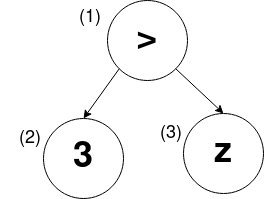
\includegraphics[scale=0.4]{FMI2.png}
\end{center}

\end{frame}



\begin{frame}{Egraphs}

\begin{itemize}
    \item refer to node $i$ by its number using $N(i)$ or its term e.g. $N(k+1)$
    \item black arrows define edges
    \item order of black arrows from left to right defines the order of the children
    \item red dotted arrows define equivalence classes
    
\end{itemize}
\pause

$\varphi_1 (x,y,z) \triangleq z \approx read(a,x) \land k + 1 \approx read(a,y) \land x \approx y \land 3 > z$

\begin{center}
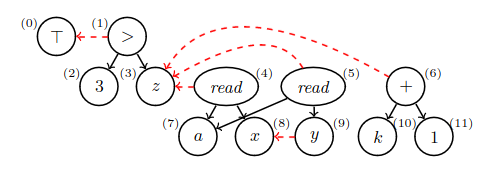
\includegraphics[scale=0.5]{FMI1.png}
\end{center}

\end{frame}


\begin{frame}{Extracting Formulas from Egraphs}
    \begin{itemize}
        \item representative functions
        \begin{itemize}
            \item $repr$ assigns each class a unique representative node
            \item example: $repr_1 \triangleq \{ N(3), N(8) \}$
        \end{itemize}
        \item \textbf{$ntt (node-to-term)$}
        \begin{itemize}
            \item extraction based on representative function repr
            \item extracts terms of a node recursively
            \item example: $ntt(N(5))$ extracts $read(a,x)$
        \end{itemize}
        \item \textbf{$to\_formula$}
        \begin{itemize}
            \item uses ntt to compute formula
        \end{itemize}
    \end{itemize}
    \begin{center}
    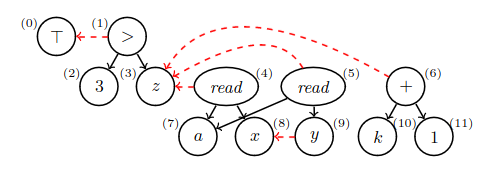
\includegraphics[scale=0.5]{FMI1.png}
    \end{center}
\end{frame}


\section{Results}

\begin{frame}{Quantifier reduction algorithm QEL}
\begin{itemize}
    \item \textbf{Input:} A formula $\varphi$ with free variables \textbf{v}.
    \item \textbf{Output:} A quantifier reduction of $\varphi$.
    \pause
    \item[1.] generating egraph from formula $\varphi$ with free variables
    \textbf{v}
    \pause
    \item[2.] computing representative function by finding ground definitions
    \pause
    \item[3.] find additional non-ground definitions
    \pause
    \item[4.] finding a core to eliminate variables
    \pause
    \item[5.] produce quantifier reduction from egraph
\end{itemize}
\end{frame}

\begin{frame}{Quantifier reduction algorithm QEL}

\begin{center}
\begin{itemize}
    \item \textbf{Input:} A formula $\varphi$ with free variables \textbf{v}. 
    \textcolor{blue}{$\varphi_1 (x,y,z) \triangleq z \approx read(a,x) \land k + 1 \approx read(a,y) \land x \approx y \land 3 > z$}
    \item \textbf{Output:} A quantifier reduction of $\varphi$.
    \textcolor{blue}{$k+1 \approx read(a,x) \land 3 > k+1$}
    \item[1.] generating egraph from formula $\varphi$ with free variables
    \textbf{v}
\end{itemize}
\end{center}
\begin{center}
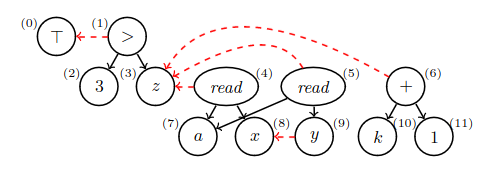
\includegraphics[scale=0.4]{FMI1.png}
\end{center}

\end{frame}

\begin{frame}{Quantifier reduction algorithm QEL}

\begin{center}
\begin{itemize}
    \item \textbf{Input:} A formula $\varphi$ with free variables \textbf{v}. 
    \textcolor{blue}{$\varphi_1 (x,y,z) \triangleq z \approx read(a,x) \land k + 1 \approx read(a,y) \land x \approx y \land 3 > z$}
    \item \textbf{Output:} A quantifier reduction of $\varphi$.
    \textcolor{blue}{$k+1 \approx read(a,x) \land 3 > k+1$}
    \item[1.] generating egraph from formula $\varphi$ with free variables
    \textbf{v}
    \item[2.] representative function by finding ground definitions
    \begin{itemize}
        \item[] \textcolor{blue}{repr = \{N(6), N(8)\}}
    \end{itemize}
\end{itemize}
\end{center}
\begin{center}
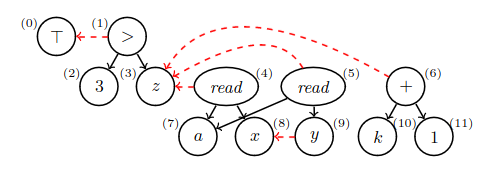
\includegraphics[scale=0.4]{FMI1.png}
\end{center}

\end{frame}

\begin{frame}{Quantifier reduction algorithm QEL}

\begin{center}
\begin{itemize}
    \item \textbf{Input:} A formula $\varphi$ with free variables \textbf{v}. 
    \textcolor{blue}{$\varphi_1 (x,y,z) \triangleq z \approx read(a,x) \land k + 1 \approx read(a,y) \land x \approx y \land 3 > z$}
    \item \textbf{Output:} A quantifier reduction of $\varphi$.
    \textcolor{blue}{$k+1 \approx read(a,x) \land 3 > k+1$}
    \item[1.] generating egraph from formula $\varphi$ with free variables
    \textbf{v}
    \item[2.] representative function by finding ground definitions
    \begin{itemize}
        \item[] \textcolor{blue}{repr = \{N(6), N(8)\}}
    \end{itemize}
    \item[3.] find additional non-ground definitions
    \begin{itemize}
        \item[] \textcolor{blue}{no refinement, repr}
    \end{itemize}
\end{itemize}
\end{center}
\begin{center}
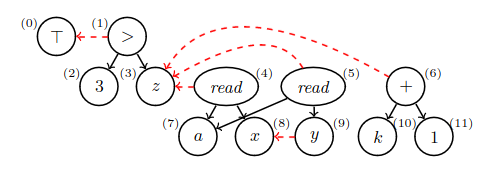
\includegraphics[scale=0.4]{FMI1.png}
\end{center}

\end{frame}

\begin{frame}{Quantifier reduction algorithm QEL}

\begin{center}
\begin{itemize}
    \item \textbf{Input:} A formula $\varphi$ with free variables \textbf{v}. 
    \textcolor{blue}{$\varphi_1 (x,y,z) \triangleq z \approx read(a,x) \land k + 1 \approx read(a,y) \land x \approx y \land 3 > z$}
    \item \textbf{Output:} A quantifier reduction of $\varphi$.
    \textcolor{blue}{$k+1 \approx read(a,x) \land 3 > k+1$}
    \item[1.] generating egraph from formula $\varphi$ with free variables
    \textbf{v}
    \item[2.] representative function by finding ground definitions
    \begin{itemize}
        \item[] \textcolor{blue}{repr = \{N(6), N(8)\}}
    \end{itemize}
    \item[3.] find additional non-ground definitions
    \begin{itemize}
        \item[] \textcolor{blue}{no refinement, repr}
    \end{itemize}
    \item[4.] finding a core to eliminate variables
    \begin{itemize}
        \item[] \textcolor{blue}{$N \setminus \{N(3), N(5), N(9) \}$}
    \end{itemize}
\end{itemize}
\end{center}
\begin{center}
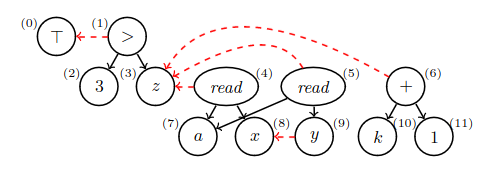
\includegraphics[scale=0.4]{FMI1.png}
\end{center}

\end{frame}

\begin{frame}{Quantifier reduction algorithm QEL}

\begin{center}
\begin{itemize}
    \item \textbf{Input:} A formula $\varphi$ with free variables \textbf{v}. 
    \textcolor{blue}{$\varphi_1 (x,y,z) \triangleq z \approx read(a,x) \land k + 1 \approx read(a,y) \land x \approx y \land 3 > z$}
    \item \textbf{Output:} A quantifier reduction of $\varphi$.
    \textcolor{blue}{$k+1 \approx read(a,x) \land 3 > k+1$}
    \item[1.] generating egraph from formula $\varphi$ with free variables
    \textbf{v}
    \item[2.] representative function by finding ground definitions
    \begin{itemize}
        \item[] \textcolor{blue}{repr = \{N(6), N(8)\}}
    \end{itemize}
    \item[3.] find additional non-ground definitions
    \begin{itemize}
        \item[] \textcolor{blue}{no refinement, repr}
    \end{itemize}
    \item[4.] finding a core to eliminate variables
    \begin{itemize}
        \item[] \textcolor{blue}{$N \setminus \{N(3), N(5), N(9) \}$}
    \end{itemize}
    \item[5.] produce quantifier reduction from egraph
    \begin{itemize}
        \item[] \textcolor{blue}{$k+1 \approx read(a,x) \land 3 > k+1$}
    \end{itemize}
\end{itemize}
\end{center}
\begin{center}
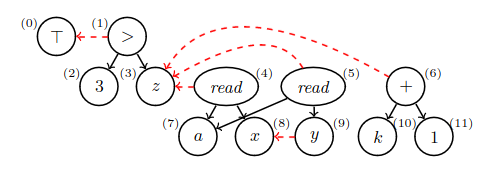
\includegraphics[scale=0.4]{FMI1.png}
\end{center}

\end{frame}

\iffalse
\begin{frame}{Quantifier reduction algorithm QEL}
\begin{itemize}
    \item computing representative function \textbf{repr} that is admissible
    \begin{itemize}
        \item finding ground definitions
        \item \textbf{find\_defs}
        \item $\Longrightarrow$ QEL found ground definitions while avoiding cycles
    \end{itemize}
    \pause
    
    \item eliminate as many variables as possible
     \begin{itemize}
        \item finding additional (non-ground) definitions
        \item \textbf{refine\_defs}
        \item $\Longrightarrow$ QEL found a representative function with as many ground definitions as possible
    \end{itemize}
    \pause
    \item finding a core of the nodes of the egraph
    \begin{itemize}
         \item \textbf{core} actually eliminates variables based on \textbf{repr}
         \item \textbf{find\_core}
    \end{itemize}
    \pause
    \item producing a quantifier elimination
    \begin{itemize}
         \item \textbf{to\_formula}
         \item $\Longrightarrow$ quantifier reduction
    \end{itemize}
   
\end{itemize}

\end{frame}
\fi

\begin{frame}{Model Based Projection MBP}
\begin{itemize}
    \item MBP was first introduced for the SPACER CHC solver for LIA and LRA (\cite{17}) and extended to the theory of Arrays (\cite{16}) and ADTs (\cite{5})
    \begin{itemize}
        \item implemented by syntactic rewriting
        \item not able to combine MBPs of multiple theories for MBP of the combination
    \end{itemize}
    \pause
    \item A model-based projection of $\varphi$ relative to $M$ is a quantifier-free formula $\psi$ s.t. $\psi \Longrightarrow \varphi^{\exists}$. Where $\varphi$ is a formula with free variables $v$ and $M$ a model of $\varphi$.
\end{itemize}
\end{frame}

\begin{frame}{MBP algorithm on top of QEL}
\begin{itemize}
  \item use MBP algorithms to project variables that cannot be eliminated cheaply
  \pause
  \item presented QEL algorithm is efficient and relatively complete but does not guarantee to eliminate all variables
  \pause
  \item use model and theory-specific projection rules to implement MBP algorithm on top of QEL
  \pause
  \item focus on Arrays and Algebraic DataTypes (ADT)
\end{itemize}
\end{frame}

\begin{frame}{MBP algorithm on top of QEL}

\begin{itemize}
    \item \textbf{Input:} A QF formula $\varphi$ with free variables \textbf{v} all of sort $Array(I,V)$ or $ADTs$, a model $M \vDash \varphi^{\exists}$, and sets of rules $ArrayRules$ and $ADTRules$
    \item  \textbf{Output:} A cube $\psi$ s.t. $\psi^{\exists} \Rightarrow \varphi^{\exists}, M \vDash \psi^{\exists}$, and $vars(\psi)$ are not Arrays or ADTs
    \pause
    \item[1.] generating egraph from formula
    \item[2.] apply MBP rules until saturation
    \item[3.] use steps of QEL to generate projected formula
\end{itemize}

\end{frame}

\begin{frame}{MBP algorithm on top of QEL}
\begin{itemize}
    \item $P \triangleq \langle A_{I \cross I}, I \rangle \dots$ datatype of a pair of an integer array and an integer
    \item $pair : A_{I \cross I} \cross I \rightarrow P$ sole constructor with destructors $fst : P \rightarrow A_{I \cross I}$ and $snd : P \rightarrow I$
    \item $i,l,j \dots$ integers
    \item $a \dots$ integer array
    \item $p,p' \dots$ pairs
    \item $p_1,p_2 \dots$ arrays of pairs
    \item $p$ and $a$ are free variables to project, all others are constants
    \item \textbf{Input:} 
    $\varphi_{mbp}(p,a) \triangleq read(a,i) \approx i \land p \approx pair(a,l) \land p_2 \approx write(p_1, j, p) \land p \not\approx p'$
\end{itemize}

\end{frame}


\begin{frame}{MBP algorithm on top of QEL}
    \begin{itemize}
        \item \textbf{Input:} 
        $\varphi_{mbp}(p,a) \triangleq read(a,i) \approx i \land p \approx pair(a,l) \land p_2 \approx write(p_1, j, p) \land p \not\approx p'$
        \item  \textbf{Output:} $read(fst(read(p_1,j)),i) \approx i \land snd(read(p_1,j)) \approx l \land read(p_2, j) \approx pair(fst(read(p_1,j)),l) \land p_2 \approx write(p_1, j, read(p_2, j)) \land read(p_2,j) \not\approx p'$
        \pause
        \item MBP is guided by a model $M_{mbp} \vDash \varphi_{mbp}$
        \pause
        \item to eliminate $p$ and $a$ construct egraph and apply MBP rules
        \pause
        \item use Array MBP rules to rewrite $write(p_1,j,p)$ by adding the equality $read(p_2, j) \approx p$ and merge it with equivalence class $p_2 \approx write(p_1,j,p)$
        \pause
        \item use ADT MBP rules to deconstruct equality $p \approx pair(a,l)$ by creating $fst(p) \approx a$ and $snd(p) \approx l$
    \end{itemize}
\end{frame}


\section{Evaluations}

\begin{frame}{QEL and MBP-QEL in Z3}
\begin{itemize}
  \item implementation publicly available \url{https://github.com/igcontreras/z3/tree/qel-cav23}
  \item Z3EG replaces QELITE with QEL and the existing MBL with MBP-QEL
  \pause
  \item evaluate Z3EG using two solving tasks
  \begin{itemize}
      \item QSAT algorithm for checking satisfiability of formulas with alternating quantifiers
      \item efficacy of MBP-QEL for Arrays and ADTs in the context of CHC-solving
  \end{itemize}
\end{itemize}
\end{frame}

\begin{frame}{QSAT algorithm for checking satisfiability of formulas with
alternating quantifiers}

\begin{itemize}
    \item in QSAT both QELITE and MBP used to under-approximate quantified formulas
    \item three QSAT implementations compared
    \begin{itemize}
        \item existing version with QELITE and MBP
        \item existing version with egraph-based algorithms
        \item QSAT implementation in YICESQS, based on the YICES SMT solver
    \end{itemize}
\end{itemize}

\pause

\begin{center}
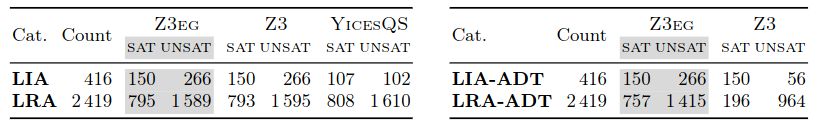
\includegraphics[scale=0.35]{FMI3.png}
\end{center}

\end{frame}

\begin{frame}{efficacy of MBP-QEL for Arrays and ADTs in the context of
CHC-solving}

\begin{itemize}
    \item Z3 uses both QELITE and MBP inside the CHC-solver SPACER
    \item comparing Z3 and Z3EG on CHC problems containing Arrays and ADTs
\end{itemize}

\pause

\begin{center}
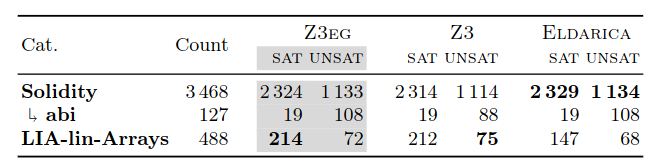
\includegraphics[scale=0.35]{FMI4.png}
\end{center}

\end{frame}


\section{Conclusion}

\begin{frame}{Conclusion}

\begin{itemize}
    \item implement directly on \textbf{egraph} data structure
    \pause
    \item resulting in easier and faster procedures
    \pause
    \item theoretical foundations for quantifier reduction
    \pause
    \item practical contributions to Z3 SMT-solver
    \pause
    \item faster than QELITE without tolerating shortcomings
\end{itemize}

\end{frame}

\section{References}

\begin{frame}[t,allowframebreaks]
    \printbibliography
\end{frame}



\end{document}
